\documentclass[tikz,border=10pt]{standalone}
\usepackage{pgfplots}
\pgfplotsset{compat=newest, scale only axis}
\providecommand{\datapath}{.}
\usepackage{xcolor}

\begin{document}
    \begin{tikzpicture}
    \begin {scope}[scale=1.25]
    \begin {scope}[scale=0.5]
        \begin{axis} [
            view ={120}{10},
            mesh/ordering=x varies,
            colorbar = true,
            colorbar style = {
                scaled ticks=false,
                ymode = log,
                log basis y=2,
                ylabel = Standard Deviation
            },
           ymajorgrids,
            xmajorgrids,
            zmajorgrids,
            xtick={0.1,0.3,0.5,0.7,0.9},
            ztick={4,16,64,256},
            ytick={0.1,0.3,0.5,0.7,0.9},
            xticklabel shift={0.15cm},
            yticklabel shift={0.15cm},
            xlabel style={sloped},
            ylabel style={sloped},
            zlabel style={sloped},
            colormap/viridis,
            width = 0.5*\textwidth,
            ylabel = $\sigma$,
            xlabel = $\rho$,
            zlabel = Mean \#Generations,
            zmode = log,
            log basis z=2,
            zmax = 256,
            clip=false
        ]

            \addplot3[surf,mesh/rows=5,opacity=0.6,colormap/viridis] table [
                x index = 1,
                y index = 0,
                z index = 2,
                point meta = \thisrowno{3},
                col sep = comma
            ] {\datapath/data/phase1_1.00.txt};
            \addplot3[surf,mesh/rows=5,opacity=0.15,colormap/viridis] table [
                x index = 1,
                y index = 0,
                z index = 2,
                point meta = \thisrowno{3},
                col sep = comma
            ] {\datapath/data/phase1_0.80.txt};
            \addplot3[surf,mesh/rows=5,opacity=0.15,colormap/viridis] table [
                x index = 1,
                y index = 0,
                z index = 2,
                point meta = \thisrowno{3},
                col sep = comma
            ] {\datapath/data/phase1_0.60.txt};
            \addplot3[surf,mesh/rows=5,opacity=0.15,colormap/viridis] table [
                x index = 1,
                y index = 0,
                z index = 2,
                point meta = \thisrowno{3},
                col sep = comma
            ] {\datapath/data/phase1_0.40.txt};
            \addplot3[surf,mesh/rows=5,opacity=0.15,colormap/viridis] table [
                x index = 1,
                y index = 0,
                z index = 2,
                point meta = \thisrowno{3},
                col sep = comma
            ] {\datapath/data/phase1_0.20.txt};
            \addplot3[surf,mesh/rows=5,opacity=0.15,colormap/viridis] table [
                x index = 1,
                y index = 0,
                z index = 2,
                point meta = \thisrowno{3},
                col sep = comma
            ] {\datapath/data/phase1_0.00.txt};
           \node (A) at (axis cs:0.15,0.25,265) {$\alpha=0.0$};
           \node (B) at (axis cs:0.15,0.25,160) {$\alpha=0.2$};
           \node (C) at (axis cs:0.15,0.25,88) {$\alpha=0.4$};
           \node (D) at (axis cs:0.15,0.25,63) {$\alpha=0.6$};
           \node (D) at (axis cs:0.15,0.25,43) {$\alpha=0.8$};
           \node (D) at (axis cs:0.15,0.25,28) {$\alpha=1.0$};
                      
        \end{axis}
        
        \end{scope}
        
        \begin{scope}[xshift=0.45*\textwidth,scale=0.5]
        \begin{axis} [
            view ={0}{90},
            mesh/ordering=x varies,
            ticklabel shift={0.2cm},
            colorbar = true,
            point meta max=32,
            point meta min=1,
            xtick={0.1,0.3,0.5,0.7,0.9},
            ytick={0.1,0.3,0.5,0.7,0.9},
            colorbar style = {
                scaled ticks=false,
                ymode = log,
                log basis y=2,
                ymin = 1,
                ymax = 32,
                ylabel = Mean \#Generations
            },
            colormap/viridis,
            width = 0.5*\textwidth,
            ylabel = $\sigma$,
            xlabel = $\rho$,
            clip=false
        ]
    \addplot3[surf,shader=interp,mesh/rows=5] table [ 
          x index = 1,
          y index = 0,
          z index = 2,
          point meta = \thisrowno{2},
          col sep = comma
] {\datapath/data/phase1_1.00.txt};
\end{axis}
          \end{scope}
        \end{scope}

        
\end{tikzpicture}
    \begin{tikzpicture}
       \begin {scope}[scale=1.25]
    \begin {scope}[scale=0.5]
        \begin{axis} [
            view ={-60}{10},
            mesh/ordering=x varies,
            colorbar = true,
            colorbar style = {
                scaled ticks=false,
                ymode = log,
                log basis y=2,
                ylabel = Standard Deviation
            },
           ymajorgrids,
            xmajorgrids,
            zmajorgrids,
            xtick={0.1,0.3,0.5,0.7,0.9},
            ztick={1,2,4,8,16},
            ytick={0.1,0.3,0.5,0.7,0.9},
            xticklabel shift={0.15cm},
            yticklabel shift={0.15cm},
            xlabel style={sloped},
            ylabel style={sloped},
            zlabel style={sloped},
            colormap/viridis,
            width = 0.5*\textwidth,
            ylabel = $\sigma$,
            xlabel = $\rho$,
            zlabel = Mean \#Generations,
            zmode = log,
            log basis z=2,
            zmax = 10,
            clip=false
        ]

            \addplot3[surf,mesh/rows=5,opacity=0.6,colormap/viridis] table [
                x index = 1,
                y index = 0,
                z index = 2,
                point meta = \thisrowno{3},
                col sep = comma
            ] {\datapath/data/phase2_0.00.txt};
            \addplot3[surf,mesh/rows=5,opacity=0.2,colormap/viridis] table [
                x index = 1,
                y index = 0,
                z index = 2,
                point meta = \thisrowno{3},
                col sep = comma
            ] {\datapath/data/phase2_0.20.txt};
            \addplot3[surf,mesh/rows=5,opacity=0.2,colormap/viridis] table [
                x index = 1,
                y index = 0,
                z index = 2,
                point meta = \thisrowno{3},
                col sep = comma
            ] {\datapath/data/phase2_0.40.txt};
            \addplot3[surf,mesh/rows=5,opacity=0.2,colormap/viridis] table [
                x index = 1,
                y index = 0,
                z index = 2,
                point meta = \thisrowno{3},
                col sep = comma
            ] {\datapath/data/phase2_0.60.txt};
            \addplot3[surf,mesh/rows=5,opacity=0.2,colormap/viridis] table [
                x index = 1,
                y index = 0,
                z index = 2,
                point meta = \thisrowno{3},
                col sep = comma
            ] {\datapath/data/phase2_0.80.txt};
           \node (A) at (axis cs:0.85,0.5,3.8) {$\alpha=0.0$};
           \node (B) at (axis cs:0.85,0.5,4.2) {$\alpha=0.2$};
           \node (C) at (axis cs:0.85,0.5,4.7) {$\alpha=0.4$};
           \node (D) at (axis cs:0.85,0.5,5.5) {$\alpha=0.6$};
           \node (E) at (axis cs:0.85,0.5,8) {$\alpha=0.8$};
                      
        \end{axis}
        
        \end{scope}
        
        \begin{scope}[xshift=0.45*\textwidth,scale=0.5]
        \begin{axis} [
            view ={0}{90},
            mesh/ordering=x varies,
            ticklabel shift={0.2cm},
            colorbar = true,
            point meta max=6,
            point meta min=2,
            xtick={0.1,0.3,0.5,0.7,0.9},
            ytick={0.1,0.3,0.5,0.7,0.9},
            colorbar style = {
                scaled ticks=false,
                ymin = 2,
                ymax = 6,
                ylabel = Mean \#Generations
            },
            colormap/viridis,
            width = 0.5*\textwidth,
            ylabel = $\sigma$,
            xlabel = $\rho$,
            clip=false
        ]
    \addplot3[surf,shader=interp,mesh/rows=5] table [ 
          x index = 1,
          y index = 0,
          z index = 2,
          point meta = \thisrowno{2},
          col sep = comma
] {\datapath/data/phase2_0.00.txt};
\end{axis}
  
        \end{scope}
        \end{scope}
        
\end{tikzpicture}

\begin{tikzpicture}
       \begin {scope}[scale=1.25]
    \begin {scope}[scale=0.5]
        \begin{axis} [
            view ={-60}{10},
            mesh/ordering=x varies,
            colorbar = true,
            colorbar style = {
                scaled ticks=false,
                ylabel = Mean \#Generations
            },
           ymajorgrids,
            xmajorgrids,
            zmajorgrids,
            xtick={0.1,0.3,0.5,0.7,0.9},
            ytick={0.1,0.3,0.5,0.7,0.9},
            xticklabel shift={0.15cm},
            yticklabel shift={0.15cm},
            xlabel style={sloped},
            ylabel style={sloped},
            zlabel style={sloped},
            colormap/viridis,
            width = 0.5*\textwidth,
            ylabel = $\sigma$,
            xlabel = $\rho$,
            zlabel = Perfect Runs,
            zmax = 1000,
            clip=false
        ]

            \addplot3[surf,mesh/rows=3,opacity=0.4,colormap/viridis] table [
                x index = 1,
                y index = 0,
                z index = 7,
                point meta = \thisrowno{2},
                col sep = comma
            ] {\datapath/data/phase3_0.00.txt};
            \addplot3[surf,mesh/rows=3,opacity=0.4,colormap/viridis] table [
                x index = 1,
                y index = 0,
                z index = 7,
                point meta = \thisrowno{2},
                col sep = comma
            ] {\datapath/data/phase3_0.20.txt};
            \addplot3[surf,mesh/rows=3,opacity=0.4,colormap/viridis] table [
                x index = 1,
                y index = 0,
                z index = 7,
                point meta = \thisrowno{2},
                col sep = comma
            ] {\datapath/data/phase3_0.40.txt};
            \addplot3[surf,mesh/rows=3,opacity=0.4,colormap/viridis] table [
                x index = 1,
                y index = 0,
                z index = 7,
                point meta = \thisrowno{2},
                col sep = comma
            ] {\datapath/data/phase3_0.60.txt};
            \addplot3[surf,mesh/rows=3,opacity=0.4,colormap/viridis] table [
                x index = 1,
                y index = 0,
                z index = 7,
                point meta = \thisrowno{2},
                col sep = comma
            ] {\datapath/data/phase3_0.80.txt};
            \addplot3[surf,mesh/rows=3,opacity=0.8,colormap/viridis] table [
                x index = 1,
                y index = 0,
                z index = 7,
                point meta = \thisrowno{2},
                col sep = comma
            ] {\datapath/data/phase3_1.00.txt};
%           \node (A) at (axis cs:0.85,0.5,3.8) {$\alpha=0.0$};
%           \node (B) at (axis cs:0.85,0.5,4.2) {$\alpha=0.2$};
%           \node (C) at (axis cs:0.85,0.5,4.7) {$\alpha=0.4$};
%           \node (D) at (axis cs:0.85,0.5,5.5) {$\alpha=0.6$};
           \node (E) at (axis cs:0.5,0.3,1010) {$\alpha=1.0$};
                      
        \end{axis}
        
        \end{scope}
        
        \begin{scope}[xshift=0.45*\textwidth,scale=0.5]
        \begin{axis} [
            view ={0}{90},
            mesh/ordering=x varies,
            ticklabel shift={0.2cm},
            colorbar = true,
            point meta max=1000,
            xtick={0.1,0.3,0.5,0.7,0.9},
            ytick={0.1,0.3,0.5,0.7,0.9},
            colorbar style = {
                scaled ticks=false,
                ylabel = Perfect Runs,
                ymax = 1000
            },
            colormap/viridis,
            width = 0.5*\textwidth,
            ylabel = $\sigma$,
            xlabel = $\rho$,
            clip=false
        ]
    \addplot3[surf,shader=interp,mesh/rows=3] table [ 
          x index = 1,
          y index = 0,
          z index = 2,
          point meta = \thisrowno{7},
          col sep = comma
] {\datapath/data/phase3_1.00.txt};
\end{axis}
  
        \end{scope}
                \end{scope}

        
\end{tikzpicture}


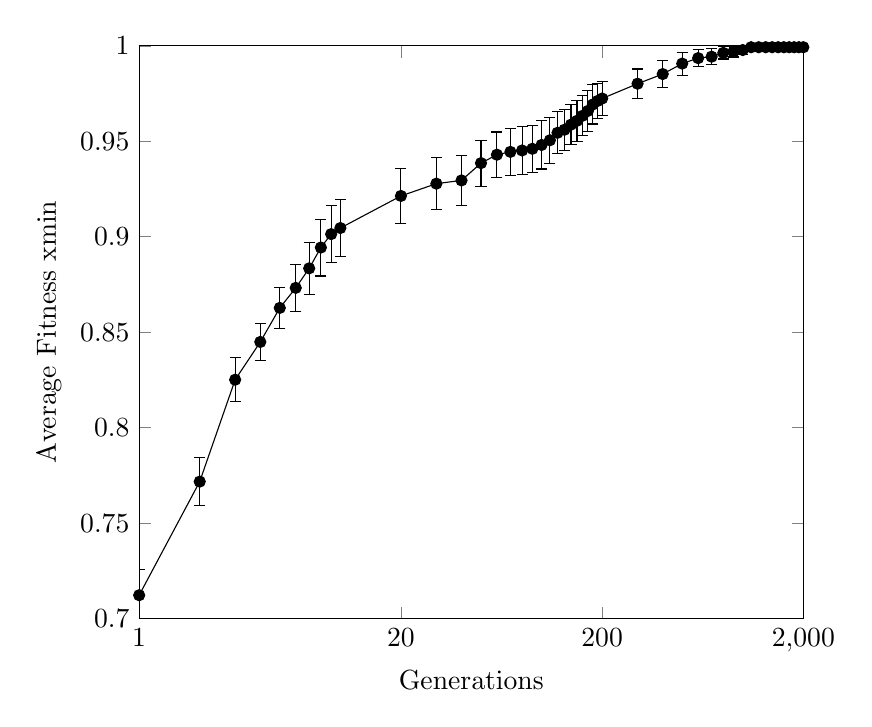
\begin{tikzpicture}
\begin{axis}[%
xlabel=Generations,
ylabel=Average Fitness
xmin=1,
xmax=2000,
xmode=log,
xtick={1, 20, 200, 2000},
enlarge y limits = false,
enlarge x limits = false,
log ticks with fixed point,
ymin=0.7,
ymax=1
]
\addplot [color=black]
 plot [mark=*, error bars/.cd, y dir = both, y explicit]
 table[row sep=crcr, x index=0, y index=1, y error index=2,]{
1 0.712276 0.013439\\
2 0.771770 0.012724\\
3 0.825130 0.011421\\
4 0.844918 0.009887\\
5 0.862741 0.010777\\
6 0.873226 0.012319\\
7 0.883469 0.013540\\
8 0.894355 0.014918\\
9 0.901385 0.014759\\
10 0.904566 0.014724\\
20 0.921372 0.014241\\
30 0.927812 0.013591\\
40 0.929507 0.013157\\
50 0.938575 0.012055\\
60 0.942976 0.011865\\
70 0.944455 0.012247\\
80 0.945194 0.012429\\
90 0.946066 0.012251\\
100 0.948068 0.012599\\
110 0.950536 0.012015\\
120 0.954443 0.010925\\
130 0.956053 0.010807\\
140 0.958712 0.010600\\
150 0.960714 0.010809\\
160 0.963372 0.010505\\
170 0.965899 0.010580\\
180 0.969296 0.010234\\
190 0.971138 0.008980\\
200 0.972401 0.008941\\
300 0.980151 0.007705\\
400 0.985204 0.006891\\
500 0.990688 0.006019\\
600 0.993561 0.004350\\
700 0.994301 0.004173\\
800 0.996303 0.003184\\
900 0.997043 0.002879\\
1000 0.997782 0.002520\\
1100 0.999261 0.001486\\
1200 0.999261 0.001486\\
1300 0.999261 0.001486\\
1400 0.999261 0.001486\\
1500 0.999261 0.001486\\
1600 0.999261 0.001486\\
1700 0.999261 0.001486\\
1800 0.999261 0.001486\\
1900 0.999261 0.001486\\
2000 0.999261 0.001486\\
};
\end{axis}
\end{tikzpicture}%

%    
%    \begin{tikzpicture}
%   \begin{scope}[scale=0.5]
%    \begin{scope}
%    
%        \begin{axis} [
%            view ={-60}{10},
%            mesh/ordering=x varies,
%            colorbar = true,
%            colorbar style = {
%                ylabel = Standard Deviation
%            },
%            colormap/viridis,
%            width = 0.5*\textwidth,
%           ymajorgrids,
%            xmajorgrids,
%            zmajorgrids,
%            xlabel style={sloped},
%            ylabel style={sloped},
%            zlabel style={sloped},
%            ylabel = Mutation Probability,
%            xlabel = Mutation Rate,
%            zlabel = Mean Iterations,
%            zmode = log,
%            zmin = 0.0,
%            zmax = 10,
%            clip=false
%        ]
%
%
%            \addplot3[surf,mesh/rows=5,opacity=0.6] table [
%                x index = 1,
%                y index = 0,
%                z index = 2,
%                point meta = \thisrowno{3},
%                col sep = comma
%            ] {\datapath/data/phase2_0.00.txt};
%            \addplot3[surf,mesh/rows=5,opacity=0.2] table [
%                x index = 1,
%                y index = 0,
%                z index = 2,
%                point meta = \thisrowno{3},
%                col sep = comma
%            ] {\datapath/data/phase2_0.20.txt};
%            \addplot3[surf,mesh/rows=5,opacity=0.2] table [
%                x index = 1,
%                y index = 0,
%                z index = 2,
%                point meta = \thisrowno{3},
%                col sep = comma
%            ] {\datapath/data/phase2_0.40.txt};
%            \addplot3[surf,mesh/rows=5,opacity=0.2] table [
%                x index = 1,
%                y index = 0,
%                z index = 2,
%                point meta = \thisrowno{3},
%                col sep = comma
%            ] {\datapath/data/phase2_0.60.txt};
%
%            \addplot3[surf,mesh/rows=5,opacity=0.2] table [
%                x index = 1,
%                y index = 0,
%                z index = 2,
%                point meta = \thisrowno{3},
%                col sep = comma
%            ] {\datapath/data/phase2_0.80.txt};
%\draw[-, gray,fill=red] (0.1,0.1,2.78) -- (0.1,0.1,73.8) node[above,black] {73.8 ($\alpha=0.0$)} circle [radius=0.035];
%\draw[-, gray,fill=orange] (0.2,0.125,2.78) -- (0.2,0.125,36.99) node[above,black] {36.99 ($\alpha=0.6$)} circle [radius=0.035];
%\draw[-, gray,fill=yellow] (0.2,0.125,2.78) -- (0.2,0.125,15.23) node[above,black] {15.23 ($\alpha=0.0$)} circle [radius=0.035];
%           \node (A) at (axis cs:0.85,0.5,3.8) {$\alpha=0.0$};
%           \node (B) at (axis cs:0.85,0.5,4.2) {$\alpha=0.2$};
%           \node (C) at (axis cs:0.85,0.5,4.7) {$\alpha=0.4$};
%           \node (D) at (axis cs:0.85,0.5,5.5) {$\alpha=0.6$};
%           \node (E) at (axis cs:0.85,0.5,8) {$\alpha=0.8$};
%
%        \end{axis}
%        
%        \end{scope}
%        
%        \begin{scope}[xshift=0.9*\textwidth]
%          \begin{axis} [
%            view ={0}{90},
%            mesh/ordering=x varies,
%            colorbar = true,
%            colorbar style = {
%                ylabel = Perfect Runs,
%                ymax = 1000
%            },
%            colormap/viridis,
%            width = 0.5*\textwidth,
%            ylabel = Mutation Probability,
%            xlabel = Mutation Rate,
%            clip=false
%        ]
%    \addplot3[surf,shader=interp,mesh/rows=3] table [ 
%          x index = 1,
%          y index = 0,
%          z index = 7,
%          point meta = \thisrowno{7},
%          col sep = comma
%] {\datapath/data/phase3_1.00.txt};
%\end{axis}
%
%        \end{scope}
%\end{scope}
%        
%    \end{tikzpicture}
%%    
%
%    \begin{tikzpicture}
%    
%    \begin{scope}[scale=0.5]
%    \begin{scope}
%        \begin{axis} [
%            view ={-60}{20},
%            mesh/ordering=x varies,
%            colorbar = true,
%            colorbar style = {
%                ylabel = Mean Iterations to Termination
%            },
%            colormap/viridis,
%            width = 0.5*\textwidth,
%           ymajorgrids,
%            xmajorgrids,
%            zmajorgrids,
%            xlabel style={sloped},
%            ylabel style={sloped},
%            zlabel style={sloped},
%            ylabel = Mutation Probability,
%            xlabel = Mutation Rate,
%            zlabel = Perfect Runs,
%            clip=false
%        ]
%
%            \addplot3[surf,mesh/rows=3,opacity=0.4] table [
%                x index = 1,
%                y index = 0,
%                z index = 7,
%                point meta = \thisrowno{2},
%                col sep = comma
%            ] {\datapath/data/phase3_0.00.txt};
%            
%            \addplot3[surf,mesh/rows=3,opacity=0.4] table [
%                x index = 1,
%                y index = 0,
%                z index = 7,
%                point meta = \thisrowno{2},
%                col sep = comma
%            ] {\datapath/data/phase3_0.20.txt};
%            \addplot3[surf,mesh/rows=3,opacity=0.4] table [
%                x index = 1,
%                y index = 0,
%                z index = 7,
%                point meta = \thisrowno{2},
%                col sep = comma
%            ] {\datapath/data/phase3_0.40.txt};
%            \addplot3[surf,mesh/rows=3,opacity=0.4] table [
%                x index = 1,
%                y index = 0,
%                z index = 7,
%                point meta = \thisrowno{2},
%                col sep = comma
%            ] {\datapath/data/phase3_0.60.txt};
%            \addplot3[surf,mesh/rows=3,opacity=0.4] table [
%                x index = 1,
%                y index = 0,
%                z index = 7,
%                point meta = \thisrowno{2},
%                col sep = comma
%            ] {\datapath/data/phase3_0.80.txt};
%            \addplot3[surf,mesh/rows=3,opacity=0.8] table [
%                x index = 1,
%                y index = 0,
%                z index = 7,
%                point meta = \thisrowno{2},
%                col sep = comma
%            ] {\datapath/data/phase3_1.00.txt};
%
%           \node (A) at (axis cs:0.85,0.5,3.8) {$\alpha=0.0$};
%           \node (B) at (axis cs:0.85,0.5,4.2) {$\alpha=0.2$};
%           \node (C) at (axis cs:0.85,0.5,4.7) {$\alpha=0.4$};
%           \node (D) at (axis cs:0.85,0.5,5.5) {$\alpha=0.6$};
%           \node (E) at (axis cs:0.85,0.5,8) {$\alpha=0.8$};
%
%        \end{axis}
%\end{scope}
%\begin{scope}[xshift=0.9*\textwidth]
%  
%
%  
%        \begin{axis} [
%            view ={0}{90},
%            mesh/ordering=x varies,
%            colorbar = true,
%            colorbar style = {
%                ylabel = Perfect Runs,
%                ymax = 1000
%            },
%            colormap/viridis,
%            width = 0.5*\textwidth,
%            ylabel = Mutation Probability,
%            xlabel = Mutation Rate,
%            clip=false
%        ]
%    \addplot3[surf,shader=interp,mesh/rows=3] table [ 
%          x index = 1,
%          y index = 0,
%          z index = 7,
%          point meta = \thisrowno{7},
%          col sep = comma
%] {\datapath/data/phase3_1.00.txt};
%\end{axis}
%\end{scope}
%\end{scope}
%\end{tikzpicture}
\end{document}